\documentclass[12pt]{article}

%%%Package Manager%%%
\setlength{\parindent}{4em}

\usepackage{amsmath}
\usepackage{setspace}
\usepackage{fancyvrb}
\usepackage{graphicx}
\usepackage{geometry}
\usepackage{hyperref}

\geometry{letterpaper, portrait, margin=1in}
%%%%%%%%%%

%%%Title Page%%%
\title{
	\begin{center}
		
\includegraphics[scale=0.5]{uga.png}\\
 	\end{center}
 	CSEE 4320 Mechatronics Systems Engineering
\bigbreak Lab 2 - Stepper Motor Lab
}

\author{
{\normalsize
\begin{tabular}{l c c}
& \textbf{Zachary Davis} & Tatsuya Kudo\\
& 811960668 & ----- \\
\textbf{Category} & Zachdav@uga.edu & Tatsuya.kudo@gmail.com\\
\hline
Lab 1: Stator \& Rotor & & 25\% \\
Lab 2: Stepper Circuit & & 25\% \\
Lab 3: Programming & & 25\% \\
Lab 4: Control & & 25\% \\
\hline
\end{tabular}
}
}

\date{\bigskip
\today}
%%%%%%%%%%

%%%Content%%%
\begin{document}
	\maketitle
	\newpage
	
	\tableofcontents
	\newpage

	\section{Lab 1: Stator \& Rotor}
		\subsection{Parts}
			\paragraph{}
				Before beginning the lab we needed to collect all the necessary parts 
				to build the rotor.  This included...\\

				\begin{itemize}
					\item 6 Neodymium Magnets
					\item 1 8mm-22mm Bearing
					\item 8 Nails
					\item 8 25ft Lengeth Magnetic Wire (200ft)
					\item 1 Arduino Uno
					\item 4 NPN Transistors (TIP3A)
					\item 1 3D Printed Rotor
					\item 1 3D Printed Stator
					\item Hot Glue
					\item 1 Compass
					\item 1 Potentiometer
					\item 1 Binary Switch
				\end{itemize}

		\subsection{3D Print the Dodecagon Rotor and Octagon Stator}
			\paragraph{}
				We used the Lutzbot 3D printer to print our rotor and stator, which was 
				accomplised in around 8 hours.

		\subsection{Magnet Polarity}
			\paragraph{}
				For this we did not have a compass that did not use GPS like the one on 
				our smart phones.  To deal with this we used our phones to determine where 
				north was then we put one magnet on a nail and put that on a bed to float 
				in water.  We then spun it and were ever it settled based on the earths 
				magnetic field we were able to determine the polarity of the magnet.  Once
				we knew one we knew them all.

		\subsection{Stator-Bearing Fitting}
			\paragraph{}
				We used our bearing by first pressing it into the stator and then pushing 
				the rotor in.  Due to the measurements of the two we were able to rely on 
				the tight fit friction to hold the bearings housing.

		\subsection{Solenoid Fabrication}
			\paragraph{}
				For the solenoid fabrication we cut 8 25ft wires and then attached a nail 
				to a drill.  After doing the first initial wraps we spun the drill to finish
				the rest of the wire sure to leave enough wire to work with in our later 
				circuit.  The dirction of spin of the wire did not matter as long as they 
				were all uniform, and we spun ours clockwise. 

		\subsection{Stepper Motor Assembly}
			\paragraph{}
				We hot glued our 6 magnets to the rotor having the south end of all the magnets 
				facing out.  We hot glued our nails in place so they were at the same height as 
				the rotor to maximize the strength of the magnetic field.

				\begin{center}
					\includegraphics[scale=0.04]{motor.jpg}\\
			 	\end{center}	

	\section{Lab 2: Stepper Circuit}
		\subsection{Solder Everything Together}
			\paragraph{}
				One thing that we were not able to get was a silcon grid to permenatly solder 
				together the circuit so we connected the coil pairs such that there polairty was 
				the same with heat shrink leaving the positive and negative end free.  Then we 
				built our circuit on a bread board and used an external power supply to power 
				the coils.  It is worth noting that we needed to use NPN transistors rather than
				PNP as labeled in the below circuit as well as transistors with a larger 
				saturation current and i can not think of way to do it any differently that 
				will work as in a PNP current can not travel out of base.

				\begin{center}
					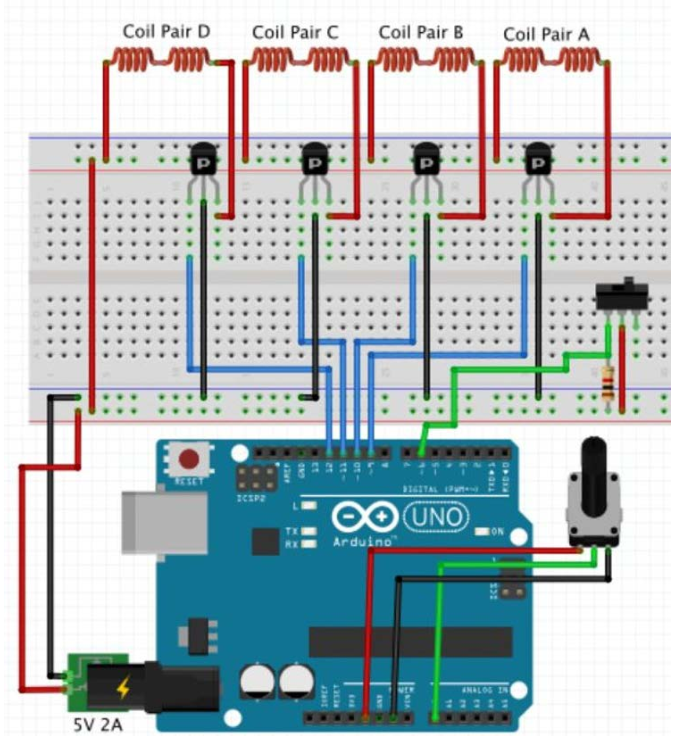
\includegraphics[scale=0.3]{circuit.png}\\
			 	\end{center}				

	\section{Lab 3: Programming}
		\subsection{Arduino Programming}
			\paragraph{}
				Below is our arduino code based on what was given to us by the instructor, where
				in one potentiometer would control the output speed of our motor and another 
				potentiometer that would control the director of spin of the rotor.  No one 
				could make the switch work that i know of.  These can be seen in the video.  It 
				is worth noting that had we had more time rather then used the provided work as 
				help i would have choosen to used the arduinos build in PWM function to actually 
				create PWM waves to the motor rathen than doing this manually.  This created clear 
				more efficient code.

				\begin{verbatim}
/*
Stepper Motor Controller
Zachary Davis & Tatsuya Kudo
October 20th, 2018
*/

//Declare Program Wide Variables
int RotationalDelay;
int reverseSwitch;

//Configure Arduino Pins
void setup(){
  
  //Solenoid Output Pins
  pinMode(9, OUTPUT);
  pinMode(10, OUTPUT);
  pinMode(11, OUTPUT);
  pinMode(12, OUTPUT);

  //Dircetion Input
  pinMode(6, INPUT);  
}

//Actual Control Loopy
void loop(){

  //Read in the value of the pot to determine dirction.
  reverseSwitch = digitalRead(6);
  
  if(reverseSwitch == LOW){
    //Read in the speed delay from pot and apply to map.
    RotationalDelay = analogRead(0);
    RotationalDelay = map(RotationalDelay, 0, 1023, 60, 2000);

    //Set which coils to be High delay and set Low.
    digitalWrite(12, HIGH);
    digitalWrite(13, HIGH);     
    delay(RotationalDelay);           
    digitalWrite(12, LOW);
    digitalWrite(13, LOW); 
    delay(5);

    //This is repeated 3 more times for all coils
    RotationalDelay = analogRead(0);
    RotationalDelay = map(RotationalDelay, 0, 1023, 60, 2000);
  
    digitalWrite(11, HIGH); 
    delay(RotationalDelay);           
    digitalWrite(11, LOW); 
    delay(5);
  
    RotationalDelay = analogRead(0);
    RotationalDelay = map(RotationalDelay, 0, 1023, 60, 2000);
  
    digitalWrite(10, HIGH); 
    digitalWrite(13, HIGH);  
    delay(RotationalDelay);           
    digitalWrite(10, LOW);
    digitalWrite(13, LOW); 
    delay(5);
  
    RotationalDelay = analogRead(0);
    RotationalDelay = map(RotationalDelay, 0, 1023, 60, 2000);
  
    digitalWrite(9, HIGH); 
    delay(RotationalDelay);           
    digitalWrite(9, LOW); 
    delay(5);   
  }
  else{
    //This is the same as above although in the opposite direction.
    RotationalDelay = analogRead(0);
    RotationalDelay = map(RotationalDelay, 0, 1023, 60, 2000);
      
    digitalWrite(9, HIGH);
    digitalWrite(13, HIGH);     
    delay(RotationalDelay);           
    digitalWrite(9, LOW);
    digitalWrite(13, LOW); 
    delay(5);
    
    RotationalDelay = analogRead(0);
    RotationalDelay = map(RotationalDelay, 0, 1023, 60, 2000);
    
    digitalWrite(10, HIGH); 
    delay(RotationalDelay);           
    digitalWrite(10, LOW); 
    delay(5);
    
    RotationalDelay = analogRead(0);
    RotationalDelay = map(RotationalDelay, 0, 1023, 60, 2000);
    
    digitalWrite(11, HIGH); 
    digitalWrite(13, HIGH);  
    delay(RotationalDelay);           
    digitalWrite(11, LOW);
    digitalWrite(13, LOW); 
    delay(5);
    
    RotationalDelay = analogRead(0);
    RotationalDelay = map(RotationalDelay, 0, 1023, 60, 2000);
    
    digitalWrite(12, HIGH); 
    delay(RotationalDelay);           
    digitalWrite(12, LOW); 
    delay(5);
  }  
}
				\end{verbatim}
	\newpage
	
	\section{Lab 4: Control}
		\subsection{Final Test}
			\paragraph{}
				Below is a photo of the group and our motor and circuit along with a link to a 
				video of our motor in operation.
				
				\begin{center}
					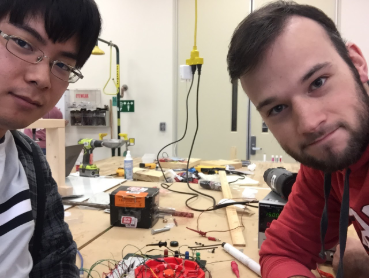
\includegraphics[scale=1]{group.png}\\
					\href{https://drive.google.com/open?id=1j-WZYNuP84D8nHtVURSW0-cqH5gjiNzz}
					{Stepper Motor in Operation}\\
					\vspace{5mm}
					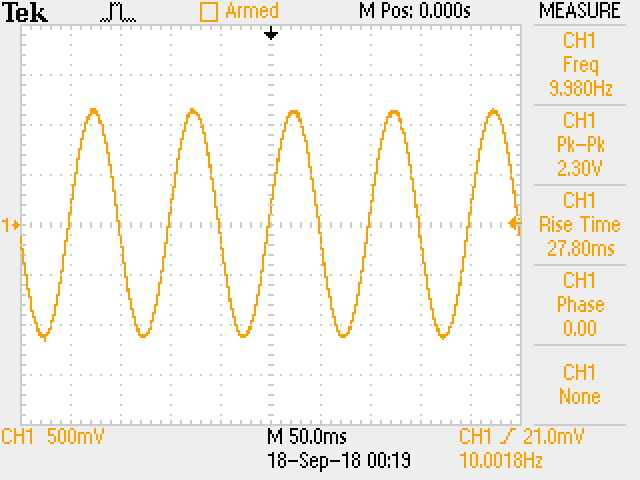
\includegraphics[scale=0.8]{output.png}\\
			 	\end{center}

			 	Our motors angular resoultion is $15^\circ$ and our maximum rotational speed is
			 	recorded at 0.0066667 RPMs.  It is the output voltage of the potentiometer that 
			 	determies the delay map which directly relates to RPM.  Our RPM could be much 
			 	greater if we spent more time with the map and optimized the materials weights
			 	and magnetic flux.
\end{document}
%%%%%%%%%%